\documentclass[preprint,12pt,aps,pra,showkeys,amsmath,amssymb,superscriptaddress,floatfix]{revtex4-2}
\usepackage[T1]{fontenc}
\usepackage[utf8]{inputenc}
\usepackage{amsmath,amssymb,amsthm,mathtools,mathrsfs}
\usepackage{microtype,booktabs,enumitem}
\usepackage{xcolor,tikz,etoolbox}
\usepackage[skins,breakable]{tcolorbox}
\usepackage{needspace}
% Keep diagram geometry independent of REVTeX preprint body spacing.
\AtBeginEnvironment{tikzpicture}{\linespread{1}\selectfont}
\usetikzlibrary{arrows.meta,positioning,calc,fit,decorations.pathreplacing}
\usepackage{graphicx}
\usepackage{hyperref}

\definecolor{MMBlue}{RGB}{0,82,155}
\definecolor{MMOrange}{RGB}{200,80,0}
\tikzset{
 mmnode/.style={draw=MMBlue,rounded corners=2pt,fill=MMBlue!4,align=left,execute at begin node={\raggedright},text width=5cm,font=\fontsize{10}{12}\selectfont,inner sep=6pt},
 mmimport/.style={mmnode,draw=black!65,fill=black!4},
 mmcandidate/.style={mmnode,draw=MMOrange,dashed,fill=MMOrange!5},
 mmrejected/.style={mmnode,draw=black,densely dotted,fill=black!8},
 mmproof/.style={->,thick,MMBlue},
 mmflow/.style={->,semithick,black!70},
 mmrepair/.style={->,dashed,thick,MMOrange},
 mmcandidatearrow/.style={->,dashed,semithick,MMOrange},
 mmnote/.style={font=\scriptsize,fill=white,inner sep=2pt,align=center}}

\usepackage[section]{placeins}
\setlength{\emergencystretch}{3em}
\setlist{itemsep=3pt,topsep=4pt}
\newtheorem{theorem}{Theorem}[section]
\newtheorem{proposition}[theorem]{Proposition}
\newtheorem{lemma}[theorem]{Lemma}
\newtheorem{corollary}[theorem]{Corollary}
\theoremstyle{definition}
\newtheorem{definition}[theorem]{Definition}
\newtheorem{example}[theorem]{Example}
\theoremstyle{remark}
\newtheorem{remark}[theorem]{Remark}
% Avoid isolated statement headings and single-line paragraph fragments.
\BeforeBeginEnvironment{theorem}{\Needspace{6\baselineskip}}
\BeforeBeginEnvironment{definition}{\Needspace{5\baselineskip}}
\BeforeBeginEnvironment{proposition}{\Needspace{5\baselineskip}}
\BeforeBeginEnvironment{lemma}{\Needspace{5\baselineskip}}
\BeforeBeginEnvironment{corollary}{\Needspace{5\baselineskip}}
\clubpenalty=5000
\widowpenalty=5000
\newcommand{\R}{\mathbb R}\newcommand{\Z}{\mathbb Z}\newcommand{\N}{\mathbb N}
\newcommand{\Pa}{\operatorname{Pa}}\newcommand{\Desc}{\operatorname{Desc}}
\newcommand{\cl}{\operatorname{cl}}\newcommand{\cost}{\operatorname{cost}}
\newcommand{\status}{\operatorname{status}}
% Faculty cards: a visual rail groups the five faculties within one agent.
% The rail has no arrowhead and does not represent a proof dependency.
\newcommand{\mmfacultybadge}[1]{%
 \node[circle,draw=MMBlue,line width=1pt,fill=white,
 minimum size=7mm,inner sep=0pt,font=\sffamily\small\bfseries,text=MMBlue]
 at ([xshift=15pt,yshift=-15pt]frame.north west) {#1};}
\newcommand{\mmfacultyrail}{%
 \draw[MMBlue!80,line width=1pt]
 ([xshift=15pt,yshift=2pt]frame.north west)--
 ([xshift=15pt,yshift=-2pt]frame.south west);}
\newtcolorbox{mmfacultybox}[2]{enhanced,breakable,
 colback=MMBlue!4,colframe=MMBlue!4,boxrule=0pt,arc=3pt,
 left=39pt,right=9pt,top=4pt,bottom=4pt,
 before skip=2pt,after skip=2pt,
 fontupper=\small\linespread{1.1}\selectfont,
 overlay unbroken={\mmfacultyrail\mmfacultybadge{#1}},
 overlay first={\mmfacultyrail\mmfacultybadge{#1}},
 overlay middle={\mmfacultyrail},overlay last={\mmfacultyrail}}
\newcommand{\mmfaculty}[3]{%
 \begin{mmfacultybox}{#1}{#2}
 {\sffamily\bfseries\color{MMBlue}#2}\par\smallskip #3
 \end{mmfacultybox}}
\newcommand{\agent}[9]{%
 \Needspace{8\baselineskip}
 \subsubsection{#1}
 \noindent\textbf{Object.} #2\par
 \noindent\textbf{Role.} #3\par\smallskip
 \mmfaculty{E}{Ego}{#4}
 \mmfaculty{M}{Memory}{#5}
 \mmfaculty{I}{Intellect}{#6}
 \mmfaculty{S}{Sense}{#7}
 \mmfaculty{A}{Action}{#8}
 \smallskip\noindent #9\par}

\usepackage{longtable,array,calc}
\providecommand{\tightlist}{\setlength{\itemsep}{2pt}\setlength{\parskip}{0pt}}
\makeatletter
\def\frontmatter@abstract@produce{\par\addvspace{\frontmatter@preabstractspace}%
\begingroup\prep@absbox\unvbox\absbox\post@absbox\endgroup
\addvspace{\frontmatter@postabstractspace}}
\makeatother
\newcommand{\field}[2]{\par\smallskip\noindent\textbf{#1.} #2\par}
\setlength{\emergencystretch}{5em}
\AtBeginEnvironment{verbatim}{\small\linespread{1.0}\selectfont}


\hypersetup{colorlinks=true,linkcolor=MMBlue,urlcolor=MMBlue,pdfauthor={Dibakar Sigdel}}

\begin{document}

\title{Lebesgue Dominated Convergence Theorem\\[4pt]\large An End-to-End Meta-Math Walkthrough}

\author{Dibakar Sigdel}

\affiliation{Mindverse Computing LLC, Lynnwood, WA 98087, USA}

\date{October 2026}

\begin{abstract}

A complete authored walkthrough of lebesgue dominated convergence
theorem, with explicit mathematical contracts, local verification gates,
and reusable exports. The report presents the target theorem, declared
imports, a dependency graph, five-faculty node contracts, a continuous
proof, a worked example, and a hypothesis-repair audit. It is an
authored mathematical exposition, not a deployed-agent transcript or a
formal proof-assistant certificate.

\end{abstract}\maketitle\linespread{1.12}\selectfont

\noindent\textbf{RA-04 / Real Analysis / Report v1}

\section{Target and import contract}

\begin{theorem}

On a measure space, let measurable \(f_n\to f\) almost everywhere and
\(|f_n|\le g\) almost everywhere for all \(n\), where \(g\in L^1\) is
nonnegative. Prove \(f\in L^1\), \(\|f_n-f\|_1\to 0\), and
\(\int f_n\to\int f\). We use a measurable representative \(f\) of the
almost-everywhere limit.

\end{theorem}

\subsection{Foundations and permitted imports}

On a measure space \((X,\Sigma ,\mu )\), Fatou's lemma says
\(\int \operatorname{liminf}\) \(h_n\le \operatorname{liminf}\)
\(\int h_n\) for nonnegative measurable \(h_n\). Use countable unions of
null sets and the integral triangle inequality. For complex-valued
functions, apply measurability to real and imaginary parts; the same
absolute-value proof works.

Take \(f\) to be a measurable representative of the almost-everywhere
limit; all exceptional sets are contained in a measurable null set. This
convention avoids silently assuming the measure space is complete.

\clearpage\section{Node interaction workflow}

\begin{center}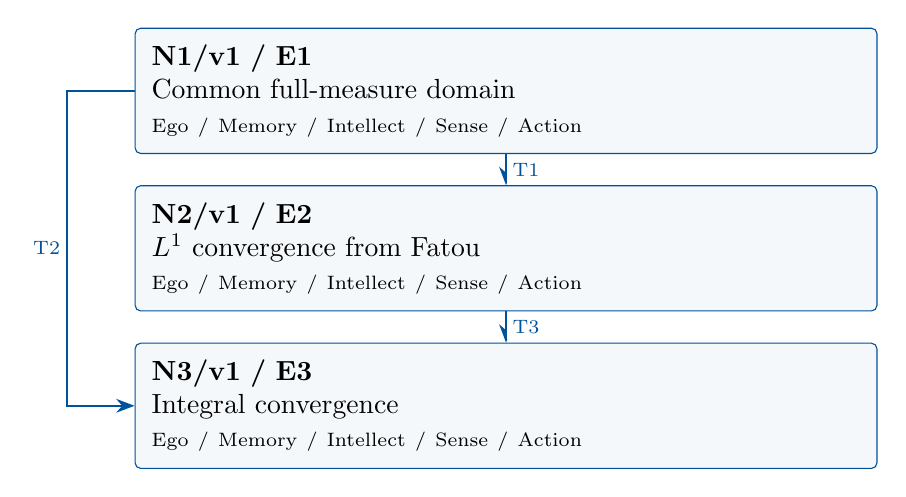
\begin{tikzpicture}[>=Stealth,x=1cm,y=1cm]

\node[mmnode,text width=9cm,minimum height=1.25cm] (N1) at (0,0.0) {\textbf{N1/v1 / E1}\\Common full-measure domain\\{\scriptsize Ego / Memory / Intellect / Sense / Action}};

\node[mmnode,text width=9cm,minimum height=1.25cm] (N2) at (0,-2.0) {\textbf{N2/v1 / E2}\\\(L^{1}\) convergence from Fatou\\{\scriptsize Ego / Memory / Intellect / Sense / Action}};

\node[mmnode,text width=9cm,minimum height=1.25cm] (N3) at (0,-4.0) {\textbf{N3/v1 / E3}\\Integral convergence\\{\scriptsize Ego / Memory / Intellect / Sense / Action}};

\draw[mmproof] (N1.south) -- node[mmnote,right] {T1} (N2.north);

\draw[mmproof] (N1.west) -- (-5.58,0) -- node[mmnote,left] {T2} (-5.58,-4) -- (N3.west);

\draw[mmproof] (N2.south) -- node[mmnote,right] {T3} (N3.north);

\end{tikzpicture}\end{center}

Each box is one mathematical agent containing all five faculties. Blue
arrows carry the versioned exports listed below. The layout gives a
reading order; only drawn arrows assert dependencies. Diagnostic repair
is separate from the proof DAG.

\subsection{Versioned evidence-transfer ledger}

\begingroup\small\linespread{1.05}\selectfont

\Needspace{5\baselineskip}\field{T1: N1/E1/v1 to N2}{The limit and all terms are integrable; all bounds hold on one
full-measure set.}

\field{Receiving activity}{N2: \(L^{1}\) convergence from Fatou}

\field{Compatibility}{Use the same mathematical objects and hypotheses as the source export.
Receiving contract: Integrable f and bounds; \(h_n=2g-|f_n-f|\); prior
exports E1/v1}

\Needspace{5\baselineskip}\field{T2: N1/E1/v1 to N3}{The limit and all terms are integrable; all bounds hold on one
full-measure set.}

\field{Receiving activity}{N3: Integral convergence}

\field{Compatibility}{Use the same mathematical objects and hypotheses as the source export.
Receiving contract: \(L^{1}\) error bound; prior exports E1/v1, E2/v1}

\Needspace{5\baselineskip}\field{T3: N2/E2/v1 to N3}{\(\Vert f_n-f\Vert _{1}\to 0\).}

\field{Receiving activity}{N3: Integral convergence}

\field{Compatibility}{Use the same mathematical objects and hypotheses as the source export.
Receiving contract: \(L^{1}\) error bound; prior exports E1/v1, E2/v1}

\endgroup

\clearpage\section{Agent roles and five-faculty activities}\begingroup\small\linespread{1.05}\selectfont\setlist{itemsep=1pt,topsep=2pt}

\subsection{N1/v1: Common full-measure domain}

\field{Object and role}{Remove all exceptional null sets at once.}

\field{Inputs}{Measurable \(f_n\); a.e. convergence; a.e. bounds \(|f_n|\le g\) with
\(g\ge 0\) integrable; foundational imports stated in §1}

\mmfaculty{E}{Ego}{Own E1/v1: The limit and all terms are integrable; all bounds hold on
one full-measure set.}

\mmfaculty{M}{Memory}{Retain Measurable \(f_n\); a.e. convergence; a.e. bounds \(|f_n|\le g\)
with \(g\ge 0\) integrable; foundational imports stated in §1; keep
their assumptions and versions attached.}

\mmfaculty{I}{Intellect}{Remove all exceptional null sets at once.}

\mmfaculty{S}{Sense}{A separate exceptional set for each n must be consolidated.}

\mmfaculty{A}{Action}{Carry out the numbered deductions and publish E1/v1 together with its
hypotheses and proof location.}

\smallskip\noindent\textbf{Numbered mathematical activities}

\begin{enumerate}[label=N1.\arabic*,leftmargin=3.4em]

\item Take the union of the convergence exceptional set and the countably many
bound exceptions.

\item It is null.

\item On its complement every bound holds and \(f_n\to f\); redefine f and
\(f_n\) on that null set if needed.

\item A pointwise limit of measurable functions is measurable, and
\(|f|\le g\) by continuity of absolute value.

\item Thus \(\int |f|\le \int g<\infty\); every \(f_n\) is integrable too.

\end{enumerate}

\field{Export E1/v1}{The limit and all terms are integrable; all bounds hold on one
full-measure set.}

\field{Acceptance gate}{A separate exceptional set for each n must be consolidated. Publish only
after checking every displayed deduction.}

\field{Targeted repair}{If the check fails, revise N1: A separate exceptional set for each n
must be consolidated. Recheck dependent nodes N2, N3.}

\clearpage

\subsection{N2/v1: \(L^{1}\) convergence from Fatou}

\field{Object and role}{Apply Fatou to a nonnegative error complement.}

\field{Inputs}{Integrable f and bounds; \(h_n=2g-|f_n-f|\); prior exports E1/v1}

\mmfaculty{E}{Ego}{Own E2/v1: \(\Vert f_n-f\Vert _{1}\to 0\).}

\mmfaculty{M}{Memory}{Retain Integrable f and bounds; \(h_n=2g-|f_n-f|\); prior exports E1/v1;
keep their assumptions and versions attached.}

\mmfaculty{I}{Intellect}{Apply Fatou to a nonnegative error complement.}

\mmfaculty{S}{Sense}{Avoid \(\infty -\infty\); finiteness of the dominating integral is used
explicitly.}

\mmfaculty{A}{Action}{Carry out the numbered deductions and publish E2/v1 together with its
hypotheses and proof location.}

\smallskip\noindent\textbf{Numbered mathematical activities}

\begin{enumerate}[label=N2.\arabic*,leftmargin=3.4em]

\item The triangle inequality gives \(0\le |f_n-f|\le 2g\), so \(h_n\ge 0\)
and \(h_n\to 2g\) almost everywhere.

\item Fatou yields
\(2\int g\le \operatorname{liminf} (2\int g-\int |f_n-f|)=2\int g-\operatorname{limsup}\)
\(\int |f_n-f|\).

\item All quantities subtracted are finite because \(g\in L^{1}\).

\item Hence the nonnegative error integrals have limsup0 and converge to 0.

\end{enumerate}

\field{Export E2/v1}{\(\Vert f_n-f\Vert _{1}\to 0\).}

\field{Acceptance gate}{Avoid \(\infty -\infty\); finiteness of the dominating integral is used
explicitly. Publish only after checking every displayed deduction.}

\field{Targeted repair}{If the check fails, revise N2: Avoid \(\infty -\infty\); finiteness of
the dominating integral is used explicitly. Recheck dependent nodes N3.}

\clearpage

\subsection{N3/v1: Integral convergence}

\field{Object and role}{Control the integral difference by its absolute error.}

\field{Inputs}{\(L^{1}\) error bound; prior exports E1/v1, E2/v1}

\mmfaculty{E}{Ego}{Own E3/v1: \(\int f_n\to \int f\), with \(f\in L^{1}\) and \(L^{1}\)
convergence.}

\mmfaculty{M}{Memory}{Retain \(L^{1}\) error bound; prior exports E1/v1, E2/v1; keep their
assumptions and versions attached.}

\mmfaculty{I}{Intellect}{Control the integral difference by its absolute error.}

\mmfaculty{S}{Sense}{Pointwise convergence alone is not the gate for an integral exchange.}

\mmfaculty{A}{Action}{Carry out the numbered deductions and publish E3/v1 together with its
hypotheses and proof location.}

\smallskip\noindent\textbf{Numbered mathematical activities}

\begin{enumerate}[label=N3.\arabic*,leftmargin=3.4em]

\item Linearity and the triangle inequality imply
\(|\int f_n-\int f|=|\int (f_n-f)|\le \int |f_n-f|\to 0\).

\item This proves the full contract, including integrability of the limit.

\item The proof does not claim pointwise convergence at exceptional points or
uniform convergence.

\end{enumerate}

\field{Export E3/v1}{\(\int f_n\to \int f\), with \(f\in L^{1}\) and \(L^{1}\) convergence.}

\field{Acceptance gate}{Pointwise convergence alone is not the gate for an integral exchange.
Publish only after checking every displayed deduction.}

\field{Targeted repair}{If the check fails, revise N3: Pointwise convergence alone is not the
gate for an integral exchange. Withhold this terminal result until its
gate passes.}

\endgroup\clearpage\section{Continuous mathematical proof}\label{sec:proof}

Read these steps in order as one proof; the diagram is optional.
Numbered activities identify the specific constructions and deductions
owned by each node.

\subsection{§4.N1 --- Common full-measure
domain}\label{n1-common-full-measure-domain}

\begin{enumerate}
\def\labelenumi{\arabic{enumi}.}
\item
  Take the union of the convergence exceptional set and the countably
  many bound exceptions.
\item
  It is null.
\item
  On its complement every bound holds and \(f_n\to f\); redefine f and
  \(f_n\) on that null set if needed.
\item
  A pointwise limit of measurable functions is measurable, and
  \(|f|\le g\) by continuity of absolute value.
\item
  Thus \(\int |f|\le \int g<\infty\); every \(f_n\) is integrable too.
\end{enumerate}

Define \(h_n=2g-|f_n-f|\ge0\) after modifying on the common measurable
null set.

\subsection{\texorpdfstring{§4.N2 --- \(L^{1}\) convergence from
Fatou}{§4.N2 --- L\^{}\{1\} convergence from Fatou}}\label{n2-l1-convergence-from-fatou}

\begin{enumerate}
\def\labelenumi{\arabic{enumi}.}
\item
  The triangle inequality gives \(0\le |f_n-f|\le 2g\), so \(h_n\ge 0\)
  and \(h_n\to 2g\) almost everywhere.
\item
  Fatou yields
  \(2\int g\le \operatorname{liminf} (2\int g-\int |f_n-f|)=2\int g-\operatorname{limsup}\)
  \(\int |f_n-f|\).
\item
  All quantities subtracted are finite because \(g\in L^{1}\).
\item
  Hence the nonnegative error integrals have limsup0 and converge to 0.
\end{enumerate}

\subsection{§4.N3 --- Integral
convergence}\label{n3-integral-convergence}

\begin{enumerate}
\def\labelenumi{\arabic{enumi}.}
\item
  Linearity and the triangle inequality imply
  \(|\int f_n-\int f|=|\int (f_n-f)|\le \int |f_n-f|\to 0\).
\item
  This proves the full contract, including integrability of the limit.
\item
  The proof does not claim pointwise convergence at exceptional points
  or uniform convergence.
\end{enumerate}

\hfill$\square$

\section{Worked orchestration}

On{[}0,1{]}, \(f_n(x)=x^{n}\) is dominated by 1 and converges to 0
except at \(x=1\). Thus \(f=0\) as an \(L^{1}\) class;
\(\int x^{n}=1/(n+1)\to 0\), matching the theorem. Uniform convergence
fails because the supremum remains1.

\subsection{Boundary and hypothesis audit}

\(On(0,1)\), \(f_n=n\cdot 1_{0,1/n}\) converges pointwise to 0 while
\(\int f_n=1\). If an \(L^{1}\) dominator existed DCT would contradict
this calculation; directly its required lower bounds force nonintegrable
growth near0. Sense blocks the common-dominator claim rather than
modifying the limit calculation.

\section{Illustrative failure and repair}

The following is an authored diagnostic scenario. Changed assumptions
define a new contract; they do not retroactively prove the original
statement.

\subsection{Failure and correction}
This is an authored teaching trace, not a recorded agent run.

\begin{enumerate}
\def\labelenumi{\arabic{enumi}.}
\tightlist
\item
  \textbf{Ego \(\to\) Memory:} register the §1 theorem, imports, and
  requested exports before beginning the proof.
\item
  \textbf{Intellect \(\to\) Action:} choose the bridges in §3 and carry
  out the numbered activities in §4; transmit only established E-exports
  along the §2 DAG.
\item
  \textbf{Sense \(\to\) responsible node:} test the specific
  boundary/failure in §5 and the node's individual audit. A failing
  candidate is withheld; downstream nodes may not use it.
\item
  \textbf{Memory + Intellect:} identify whether the error is an omitted
  condition, an invalid inference, or an attempted extension beyond the
  theorem. Restore the exact contract or explicitly state a different
  one.
\item
  \textbf{Action:} redo the affected mathematical activity using the
  repaired condition or inference. Recheck consuming nodes, rather than
  feeding their conclusions back as premises.
\item
  \textbf{Ego:} publish only the supported export with its assumptions
  and proof location. A hypothetical revised export is v2; the written
  proof here is the v1 exposition, not a claim that this repair was
  executed.
\end{enumerate}

\subsection{Hypothesis boundary}
\(On(0,1)\), \(f_n=n\cdot 1_{0,1/n}\) converges pointwise to 0 while
\(\int f_n=1\). If an \(L^{1}\) dominator existed DCT would contradict
this calculation; directly its required lower bounds force nonintegrable
growth near0. Sense blocks the common-dominator claim rather than
modifying the limit calculation.

\subsection{Version and recheck}
Treat any changed assumption as a new contract. Recheck the revised
export and all of its descendants. A backward diagnostic never
establishes an earlier theorem. This is an authored teaching trace, not
an execution log.

\par\medskip\begingroup\small\linespread{1.0}\selectfont\noindent\textbf{Provenance.} This authored proof is complete relative to its declared imports. Reuse
each export with its assumptions, proof, and version. The original
Markdown remains available for comparison.
\par\endgroup

\par\smallskip\begingroup\small\linespread{1.0}\selectfont\noindent\textbf{Further reading.} \begin{itemize}
\tightlist
\item
  \href{https://ocw.mit.edu/courses/18-125-measure-and-integration-fall-2003/pages/lecture-notes/}{Fatou
  and dominated convergence: MIT Measure and Integration}.
\end{itemize}\par\endgroup

\end{document}
